\mysubsubsection{Layered Depthmap}

\begin{figure}[tb]
  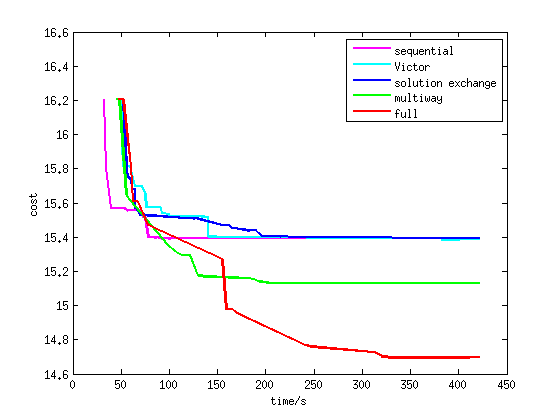
\includegraphics[width=\columnwidth]{figure/layered_depthmap_convergence.png}
  \caption{The energy minimization process for layered depthmap estimation of different methods. Multi-way fusion is shown to be more effectvie than binary fusion in this problem setting.}\label{fig:layered_depthmap_convergence}
\end{figure}
\begin{figure}[tb]
  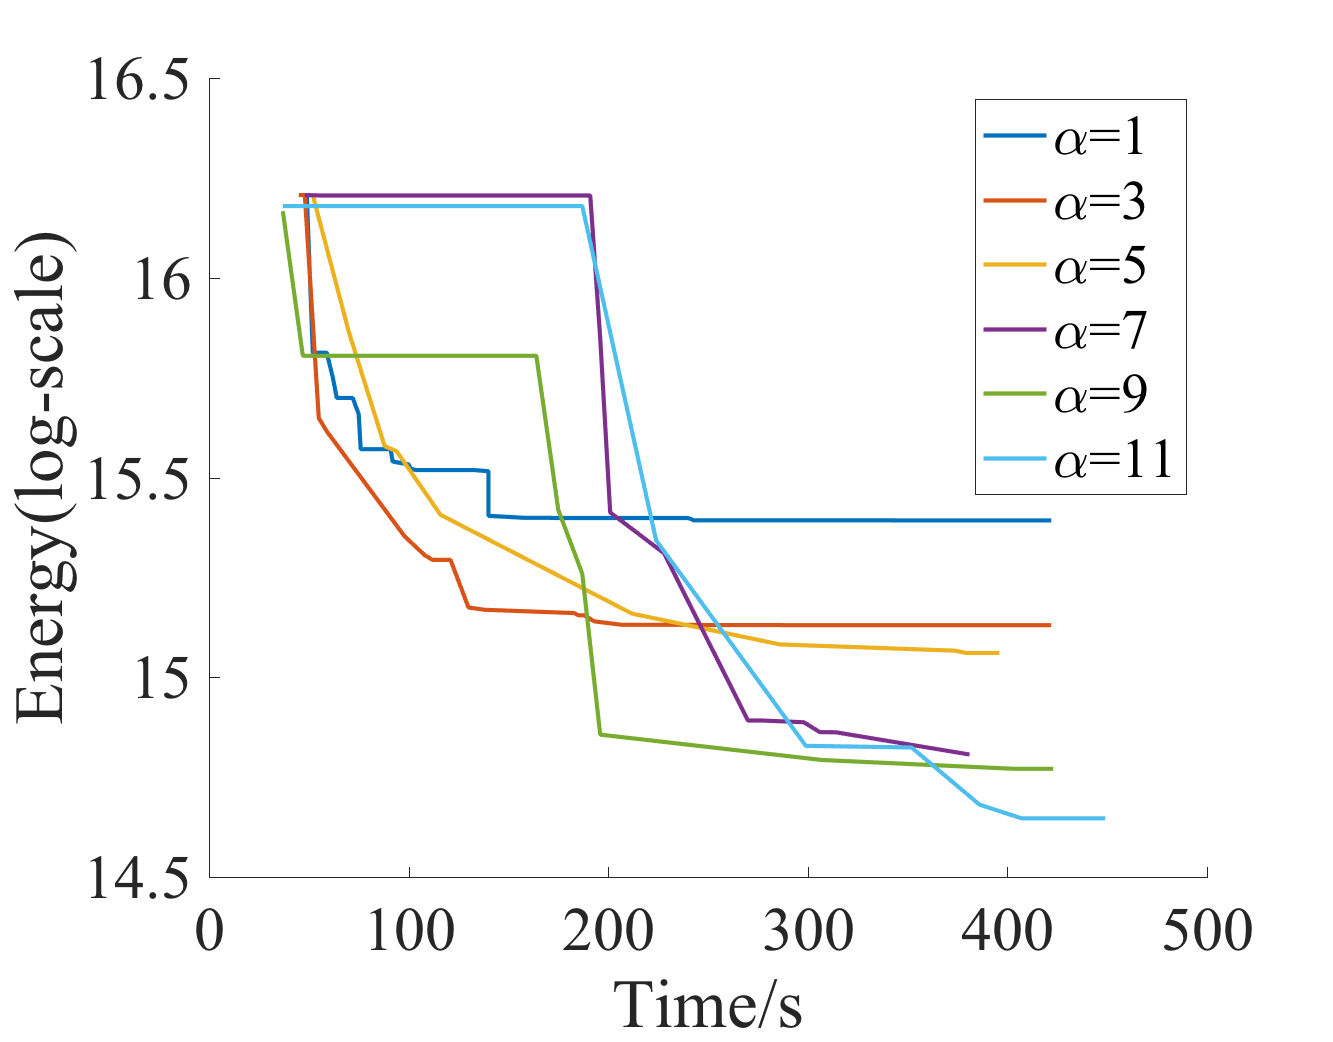
\includegraphics[width=\columnwidth]{figure/layered_depthmap_by_alpha.png}
  \caption{The energy minimization process for layered depthmap estimation with different $\alpha$ values. Multi-way fusion generally performs better than binary fusion, but the optimization becomes harder for using more ways in each step.}\label{fig:layered_depthmap_by_alpha}
\end{figure}

From the convergence plot of layered depth map estimation, we can see that, Fusion Move, Parallel Fusion Move, and FS-MF all stalk at a high energy state. The reason is binary fusion of solution proposals (either from others or self) is too limited to further decrease the energy due to the complexity of the problem itself. Only when multi-way fusion is used (in FS-SS and FS), it becomes possible for the energy to further decrease. This coincides with the observation in \cite{layered_depthmap} that binary fusion of proposal solutions is not as powerful as their subspace fusion which is a special form of multi-way fusion here. To further explore the effect of multi-way fusion, we use different $\alpha$ {1, 3, 7, 15} in FS model while keeping other parameters the same and plot the energy-time curve in figure \ref{fig:layered_depth_map_by_alpha}.

As shown in \ref{section:results}, the multi-way fusion and solution sharing enabled by our uniform framework play a key role for improving performance in different settings. For better understanding our framework, we examine the role played by each factor more closely by varying each factor while keeping others the same.

